%!TeX root = ../main.tex

% ==========================================
% CHAPTER 3: SYSTEM ARCHITECTURE AND ROS 2 SETUP
% ==========================================
\chapter{System Architecture and Infrastructure Development}
\label{ch:architecture}

This chapter details the software architecture, the simulation environment setup, and the extensive infrastructural modifications required to execute a fair and rigorous comparative analysis. The default packages provided by the manufacturer were fundamentally tailored for differential drive operations. Consequently, a significant systems engineering effort was necessary to decouple the hardcoded dependencies, resolve simulation rendering and physics engine artifacts, and fine-tune the navigation algorithms for holonomic mobility.

\section{The ROS 2 Framework and Nav2 Stack}

The software architecture of this thesis is built upon the Robot Operating System 2 (ROS 2), specifically the \textit{Humble Hawksbill} distribution. Within this framework, autonomous navigation is governed by the Navigation 2 (Nav2) stack. Nav2 is a highly modular, behavior-tree-based navigation system, conceptually divided into several distinct servers. To establish a rigorous baseline for the comparative analysis, the following specific algorithmic configurations were selected:

\begin{itemize}
    \item \textbf{Planner Server:} Computes the optimal global path from the robot's current position to a goal pose using the global costmap. For this work, the \texttt{NavfnPlanner} was employed. In the waypoint-navigation experiments it was run in Dijkstra mode (\texttt{use\_astar: false}), which performs a full wavefront expansion and returns the minimum-cost geometric path. For the autonomous-exploration experiments, where the planner is repeatedly queried for distant frontier goals, the A* heuristic was instead enabled (\texttt{use\_astar: true}) to reduce the expansion cost of each planning query.
    \item \textbf{Controller Server:} Acts as the local planner, computing the immediate velocity commands ($\vec{v} = [v_x, v_y, \omega]^T$) required to follow the global path while dynamically avoiding local obstacles. The \texttt{DWBLocalPlanner} was selected for this core task.
    \item \textbf{Behavior Server:} Manages recovery behaviors (such as clearing costmaps, backing up, or spinning in place) when the robot detects a failure or gets stuck in complex environments.
    \item \textbf{AMCL (Adaptive Monte Carlo Localization):} A probabilistic localization system that utilizes a particle filter to track the robot's pose against a known map, comparing the expected environmental geometry with real-time LiDAR scans.
\end{itemize}

The localization component depends on the experimental campaign. In the \\ waypoint-navigation experiments the map of the environment is known in advance, and the robot pose is tracked by AMCL as described above. In the autonomous-exploration experiments, by contrast, no prior map is available: localization and mapping are performed simultaneously by \texttt{slam\_toolbox} running in \texttt{mapping} mode, which incrementally builds the occupancy grid from LiDAR scan matching (using a Ceres-based pose-graph back-end) and feeds it to the Nav2 costmaps. The two campaigns therefore rely on two distinct localization regimes---AMCL on a known map for waypoint navigation, and online simultaneous localisation and mapping (SLAM) for exploration---a distinction that must be kept in mind when comparing the pose-related metrics of the two tasks.

The choice of the \texttt{DWBLocalPlanner} as the local controller is particularly significant for this study. Because its architectural legacy is a direct evolution of the Dynamic Window Approach (DWA), it inherently embodies the differential-drive bias prevalent in current industry standards. Employing it as the baseline provides a concrete starting point to evaluate the behavior of holonomic kinematics under legacy constraints, mathematically highlighting the necessity of holonomic-specific tuning.

\section{The TIAGo Robotic Platform}

The experimental evaluations are conducted using the TIAGo robot, developed by PAL Robotics. TIAGo is a highly modular service robot featuring a 7-DOF manipulator arm, a lifting torso, and an array of perception sensors mounted on its head. The critical feature of this platform, which makes it ideal for this comparative study, is its interchangeable mobile base. The upper body remains identical, ensuring that payload, sensor placement, and center of mass distributions are largely consistent, thereby isolating the kinematic drive as the primary variable.

\subsection{Differential Drive Configuration (PMB2)}
The default configuration employs the PAL Mobile Base 2 (PMB2, Figure~\ref{fig:PMB2 base}) \cite{pal_tiago_base}. This non-holonomic base is characterized by a two-wheel differential drive mechanism supported by caster wheels. 
From a software and collision-avoidance perspective, the PMB2 is modeled with a strictly circular static footprint with a radius of $0.275$ meters. Environmental perception for obstacle avoidance and AMCL localization is achieved via a single forward-facing 2D LiDAR, whose data is broadcasted on the standard \texttt{/scan\_raw} topic.

\begin{figure}[H]
    \centering
    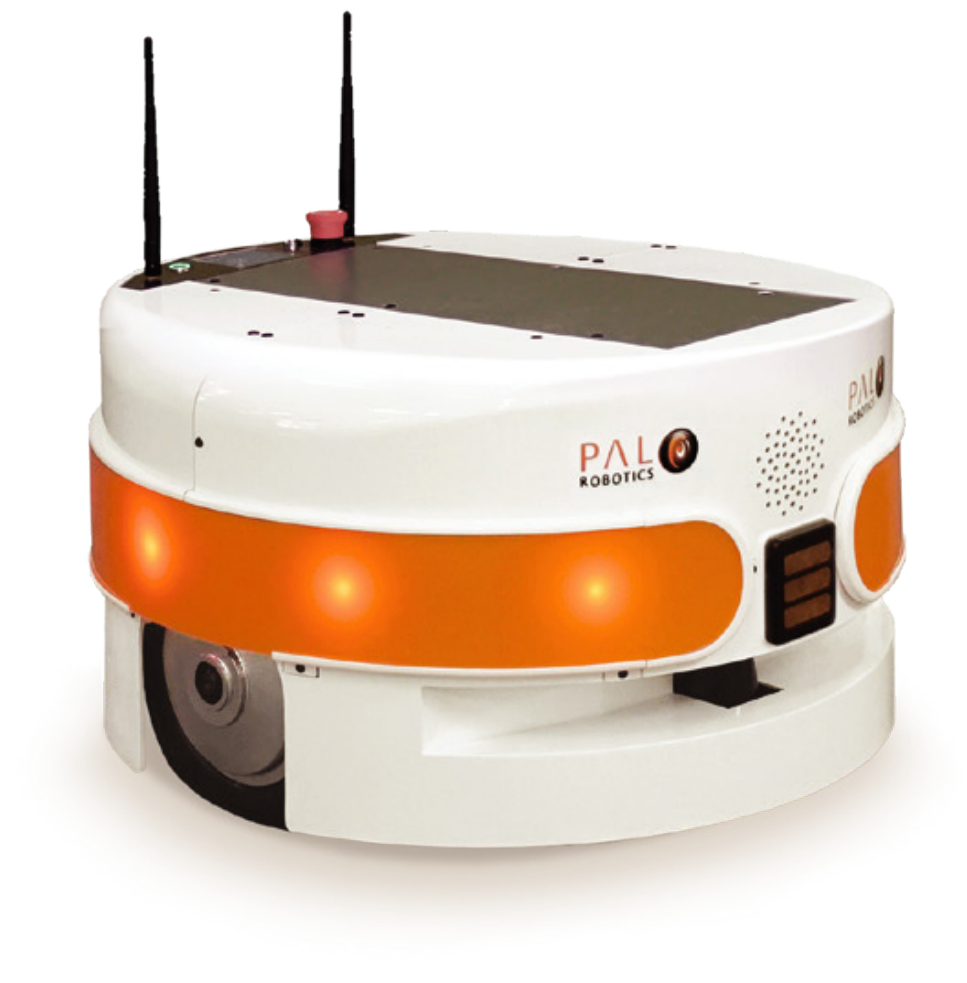
\includegraphics[width=0.4\textwidth]{images/Ch3/pmb2.png}
    \caption{PAL Robotics - PMB2 base}
    \label{fig:PMB2 base}
\end{figure}

\subsection{Omnidirectional Configuration (OmniBase)}
The alternative configuration substitutes the PMB2 with the OmniBase (Figure~\ref{fig:Omni base}) \cite{pal_tiago_omnibase}, a holonomic platform equipped with four independently driven Mecanum wheels. 
This configuration diverges significantly from the PMB2 in its physical footprint and sensory layout (Figure~\ref{fig:tiago_bases}). Due to the geometric constraints of mounting four Mecanum wheels parallel to the longitudinal axis, the OmniBase requires a rectangular footprint (defined in the local frame by the vertices \\ $[0.35, 0.24], [-0.35, 0.24], [-0.35, -0.24], [0.35, -0.24]$ in meters). Furthermore, to ensure complete 360-degree visibility without blind spots caused by the rectangular chassis, the OmniBase is equipped with two 2D LiDAR sensors, mounted diagonally (front-left and rear-right). Consequently, the sensory data is published on two distinct topics: \texttt{/scan\_front\_raw} and \texttt{/scan\_rear\_raw}.

These seemingly minor hardware differences have profound implications on the configuration of the Nav2 stack, particularly concerning footprint generation in the local and global costmaps and the correct ingestion of sensory data by the AMCL localization module.

\begin{figure}[H]
    \centering
    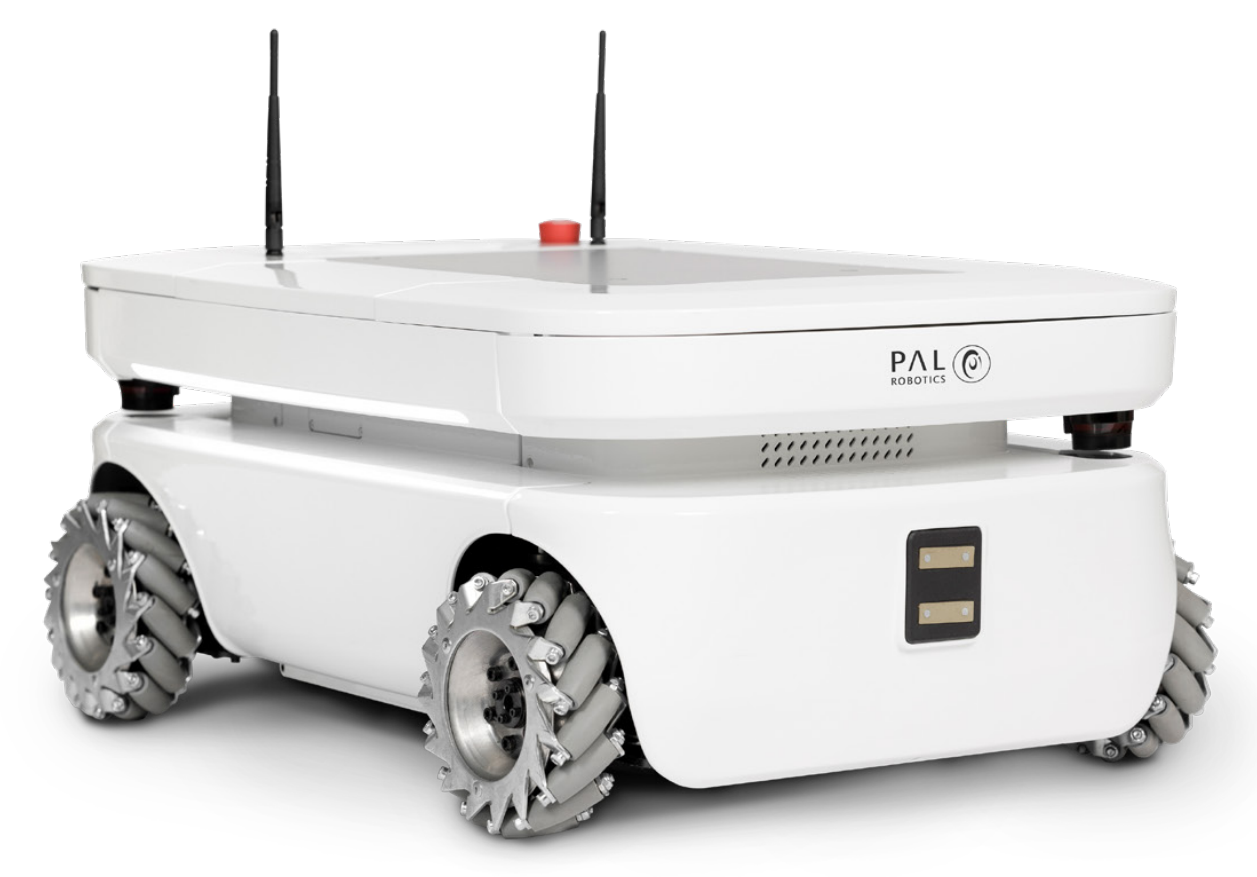
\includegraphics[width=0.4\textwidth]{images/Ch3/omni.png}
    \caption{PAL Robotics - OmniBase}
    \label{fig:Omni base}
\end{figure}

\begin{figure}[H]
     \centering
     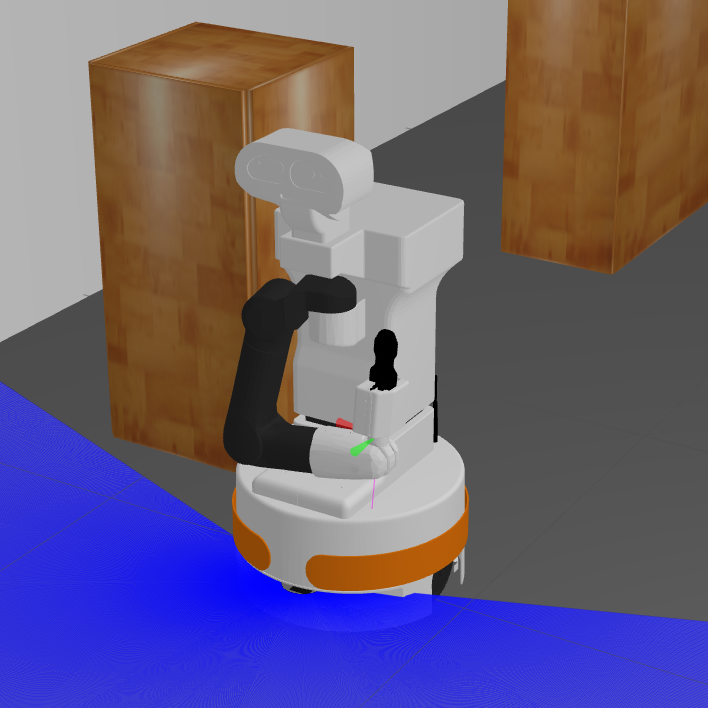
\includegraphics[width=0.45\textwidth]{images/Ch3/pmb2_gazebo.png}
     \hfill
     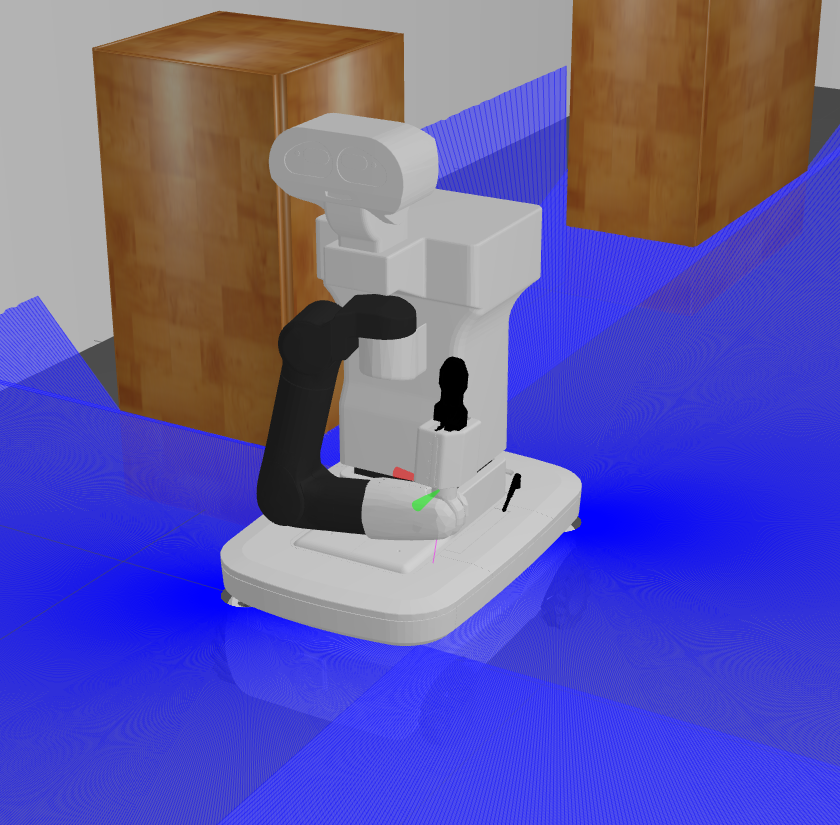
\includegraphics[width=0.45\textwidth]{images/Ch3/omni_gazebo.png}
     \caption{Comparison of the TIAGo mobile bases in Gazebo. Left: The PMB2 differential drive base. Right: The OmniBase with Mecanum wheels.}
     \label{fig:tiago_bases}
\end{figure}

\subsection{Simulation Hardware Specifications}
Because the comparative analysis heavily relies on the physical execution time and the Real-Time Factor (RTF) of the simulation, the hardware specifications of the deployment workstation must be explicitly stated to ensure scientific reproducibility. 

All experiments and simulations were executed natively on Ubuntu 22.04 LTS. The workstation is powered by an AMD Ryzen 5 3600 6-Core Processor, equipped with 32 GB of RAM, and utilizes an AMD Radeon RX 5600 XT Graphics Processing Unit. Documenting this specific GPU architecture is particularly relevant, as its direct interaction with the Gazebo OpenGL rendering pipeline motivated the environmental workarounds implemented in the subsequent section to stabilize the simulation frame rate.

\section{Workspace Setup and Simulation Fixes}
\label{sec:ws setup}

Setting up a robust simulation environment required resolving several low-level dependencies and hardware-specific bottlenecks that initially prevented the execution of the experiments.

\subsection{Dependencies and URDF Conflicts}
The provided ROS 2 workspace was initially configured exclusively for the PMB2 differential base. To enable the omnidirectional configuration, the official \texttt{omni\_base} packages were integrated into the workspace. Furthermore, the pre-installed \texttt{pal\_urdf\_utils} package originated from an unofficial repository, resulting in missing files during compilation. This was resolved by replacing it entirely with the official upstream branch.

A critical simulation failure occurred during the spawning of the TIAGo model, where the Gazebo server crashed with a segmentation fault upon initialization. Debugging revealed a namespace collision: both the standard TIAGo description and the OmniBase description attempted to instantiate an IMU plugin named \texttt{base\_imu}. To resolve this conflict, the plugin was renamed to \texttt{tiago\_base\_imu} directly within the Xacro definitions (the stream editor command used for this programmatic refactoring is provided in Appendix \ref{app:urdf_conflict}).

\subsection{GPU Rendering Optimization}
\label{subsec:gpu optimization}
During the initial testing phase on the AMD-equipped workstation, a hardware-rendering issue was identified: the physics engine failed to compute and visualize the LiDAR sensors of the OmniBase. Forcing the system to utilize CPU-based software rendering (via the \\ \texttt{LIBGL\_ALWAYS\_SOFTWARE=1} environment variable) successfully resolved the sensor computation issue. However, applying this globally caused the simulation performance to plummet to an unusable 9 Frames Per Second (FPS).

To bypass this bottleneck, a targeted bash wrapper was implemented. Instead of forcing software rendering on the entire simulation—including the graphical client (\texttt{gzclient})—the wrapper applies the variable exclusively to the Gazebo physics server (\texttt{gzserver}). The bash implementation of this targeted wrapper is documented in Appendix \ref{app:gzserver_wrapper}. This decoupling restored the simulation's viability, keeping the Real-Time Factor (RTF) in a consistent range---around $0.9$ under sustained navigation load, with short, lightly loaded runs occasionally reaching or exceeding $1.0$ (an artefact of averaging the factor over a very small time window). Because the RTF is generally at or slightly below $1.0$, the simulation clock runs at, or slightly slower than, the system wall time. It therefore became an absolute necessity to enforce and propagate the \texttt{use\_sim\_time:=true} parameter across the entire ROS~2 testing pipeline. This ensured that all nodes, controllers, and data loggers synchronised perfectly with Gazebo's internal \texttt{/clock} topic, preserving temporal consistency and guaranteeing that the comparative performance metrics remained scientifically valid regardless of the hardware-induced slowdown.

\subsection{Simulation Environments and Ground Truth Extraction}
\label{subsec:simulation_gt}
To thoroughly evaluate the platforms, two distinct Gazebo environments were utilized. For the directed waypoint navigation tests, the stock PAL Robotics \texttt{small\_office} world was used as a baseline. This environment required minor modifications to suit the benchmarking needs: the lighting was adjusted, specific obstacles like overhanging tall desks (which caused blind collisions) were removed, and static human models were added to simulate a realistic, cluttered office scenario. 
Conversely, for the autonomous exploration benchmarks, the \texttt{home} world was deployed. This environment represents a realistic domestic apartment and was left entirely unaltered to provide a highly complex scenario.

Crucially, to enable rigorous scientific evaluation, the system was configured to log the absolute Ground Truth pose of the robot across both environments. As theoretically established in Section \ref{sec:probabilistic_motion_models}, relying solely on raw odometry for error calculation would introduce an inherent estimation bias due to unbounded dead-reckoning drift. Furthermore, while localization algorithms like AMCL act to bound this drift, they inherently introduce stochastic estimation noise due to particle variance. Because the PMB2 and OmniBase generate fundamentally different probabilistic noise profiles (constrained vs. omnidirectional distributions), evaluating their path-tracking performance via their own onboard estimation would invalidate the fairness of the comparison. To ensure that the offline trajectory analyses remained strictly objective and uncontaminated by these uncertainties, the \texttt{gazebo\_ros\_state} plugin was injected into both \texttt{.world} configurations (the XML implementation of this plugin is available in Appendix \ref{app:gt_plugin}). This plugin publishes the absolute spatial coordinates of all simulated models to the ROS 2 network at a frequency of 50 Hz, providing an infallible spatial reference.

\section{The Master Launch Architecture and Dynamic Initialization}
\label{sec:launch arch}

The default launch infrastructure provided by the manufacturer lacked native support for arbitrary spawn coordinates, dynamic simulation environments, and base swapping. To systematically benchmark the two kinematic models, a custom master launch  \\ (\texttt{tiago\_thesis\_gazebo.launch.py}) was developed to orchestrate a controlled and repeatable initialization sequence, effectively acting as an initialization state-machine.

\subsection{Propagating the Kinematic Profile}
In the ROS 2 launch system, configurations are structured as an inverted tree. To allow the runtime dynamic selection of the robot's kinematics, the \texttt{base\_type} parameter was explicitly routed through the intermediate launch files down to the state publisher and controller multiplexer. The main robot description file was then refactored using conditional logic. This ensures that Gazebo dynamically assembles the correct 3D meshes, hardware controllers, and LiDAR layouts based purely on the propagated argument.

\subsection{The Odometry TF Bridge}
\label{subsec:odom tf bridge}
A critical simulation anomaly emerged exclusively when testing the OmniBase. In simulation, the holonomic base is driven by the \texttt{gazebo\_ros\_planar\_move} plugin to bypass the prohibitive computational cost of simulating physical friction on the Mecanum rollers. However, this plugin inherently bypasses the standard \texttt{ros2\_control} architecture and joint states mechanisms, failing to broadcast the essential Transform (TF) from the \texttt{odom} frame to the \texttt{base\_footprint} frame.

Because Nav2 requires a continuous TF tree, the absence of this transform causes the stack to crash upon initialization. To bridge this gap, a custom Python node (\texttt{odom\_tf\_publisher.py}) was developed to subscribe to the odometry topic and manually broadcast the missing transform (Figure~\ref{fig:tf_tree_cropped}) (the source code for this bridge is available in Appendix \ref{app:tf_bridge}). Crucially, the node was engineered to ingest the simulation time arguments, ensuring perfect temporal synchronization with the Gazebo clock. 

Beyond the missing transform, the fact that \texttt{gazebo\_ros\_planar\_move} imposes the commanded body twist directly---rather than actuating the wheels through a dynamic model, as \texttt{ros2\_control} does for the PMB2---has implications for the fairness of the kinematic comparison. These are discussed together with the evaluation metrics in Section~\ref{subsec:m-fidelity}.

\begin{figure}[H]
    \centering
    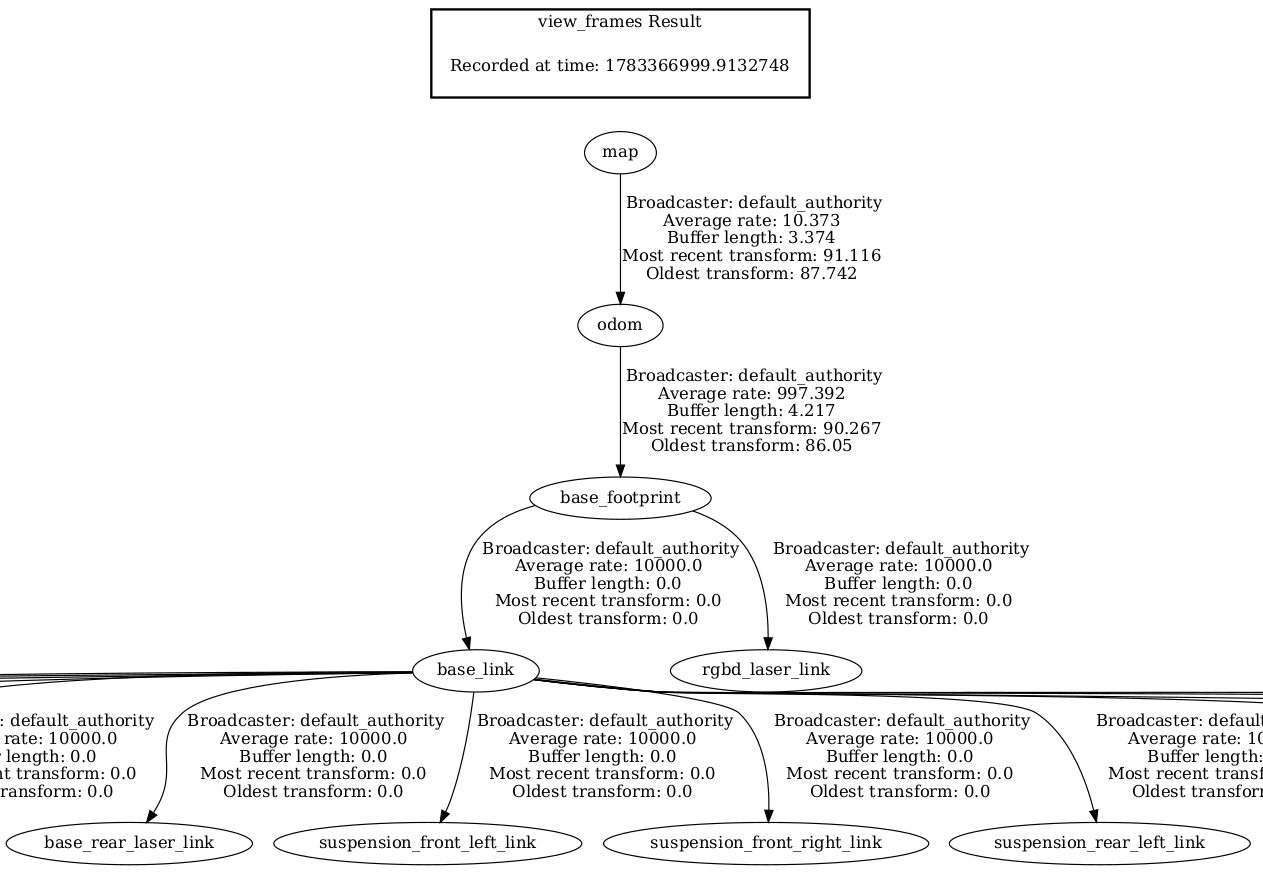
\includegraphics[width=1\textwidth]{images/Ch3/frames_diff_obs_cropped.png} 
    \caption{A heavily cropped extract of the ROS 2 TF tree for the OmniBase configuration, generated via \texttt{tf2\_tools}. The extensive kinematic branches of the upper body and auxiliary sensors have been omitted to highlight the localization root frames. Crucially, the fundamental \texttt{odom} $\rightarrow$ \texttt{base\_footprint} transform is successfully broadcasted by the custom \texttt{odom\_tf\_publisher.py} node, ensuring the continuity of the tree.}
    \label{fig:tf_tree_cropped}
\end{figure}

\subsection{Deterministic Initialization State-Machine}
\label{subsec: Deterministic Init}
To guarantee a rigorously standardized starting condition for every experimental iteration, automated routines for postural stability and spatial initialization were embedded into the launch sequence.

Spawning the TIAGo robot with its heavy 7-DOF manipulator arm fully extended creates a severe center-of-mass imbalance. Coupled with the physics engine's micro-slippage, this induces involuntary rotation upon spawning. Furthermore, since the objective of this thesis is to compare the mobile bases, an extended arm would introduce misleading spatial constraints, forcing the local planner to trigger avoidance maneuvers that do not reflect the true footprint of the base. To prevent this, the launch orchestrator actively sends a joint trajectory goal immediately at boot, transitioning the robot into a stable state by folding the arm into a compact, centralized position.

In addition to postural stability, precise spatial initialization was enforced through a dynamic teleportation routine. The orchestrator reads the user-defined coordinates and employs a robust polling loop that continually queries the ROS 2 service list (the bash implementation of this routine is detailed in Appendix \ref{app:teleport}). The teleportation payload is dispatched strictly after the physics engine fully exposes the entity manipulation service, guaranteeing that every benchmarking sequence commences from the precise mathematical coordinates required by the methodology.

\section{Navigation Stack Configuration and Algorithmic Tuning}
\label{sec:nav2_tuning}

The transition from a differential to a holonomic drive cannot be handled solely at the hardware and physics-engine levels. To conduct a fair evaluation, the Navigation 2 stack had to be profoundly reconfigured. The default parameters heavily penalize lateral movements, forcing the OmniBase into a sub-optimal "pseudo-differential" behavior. This section details the systematic parameter tuning implemented to unlock the holonomic capabilities of the OmniBase while maintaining a standardized baseline for the PMB2.

\subsection{Sensory Configuration and AMCL Probabilistic Tuning}
\label{subsec:amcl_tuning}

The physical layout of the sensors directly dictates how the robot perceives its environment and localizes itself. The differential PMB2 utilizes a single forward-facing LiDAR, whose data is broadcasted on the \texttt{/scan\_raw} topic. Conversely, to prevent blind spots along its rectangular chassis, the OmniBase relies on two LiDARs (\texttt{/scan\_front\_raw} and \texttt{/scan\_rear\_raw}). 

To ensure the \texttt{nav2\_costmap\_2d} server correctly generated the obstacle layers for the OmniBase, both the local and global costmaps were modified. The \texttt{observation\_sources} parameter was expanded to ingest both laser topics simultaneously, actively fusing the point clouds to generate a 360-degree collision map. However, because standard AMCL implementations primarily ingest a single 2D scan for particle evaluation, the localization node was explicitly routed to the primary front laser. This decoupled architectural flow is clearly visible in the active ROS 2 node graph (Figure \ref{fig:laser_graphs}).

\begin{figure}[H]
    \centering
    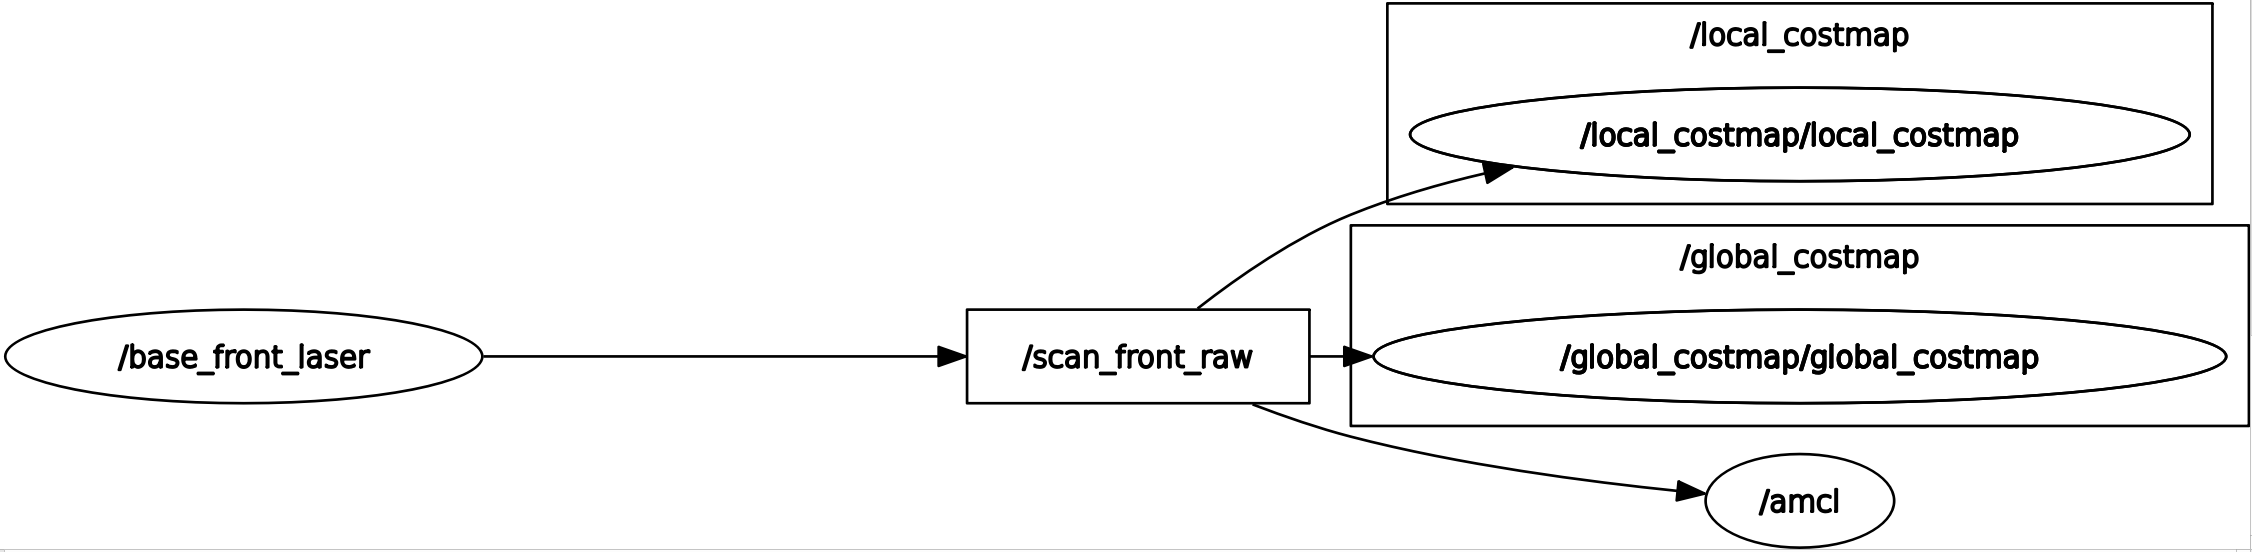
\includegraphics[width=1\textwidth]{images/Ch3/rosgraph_scan_front.png}\\[0.3cm]
    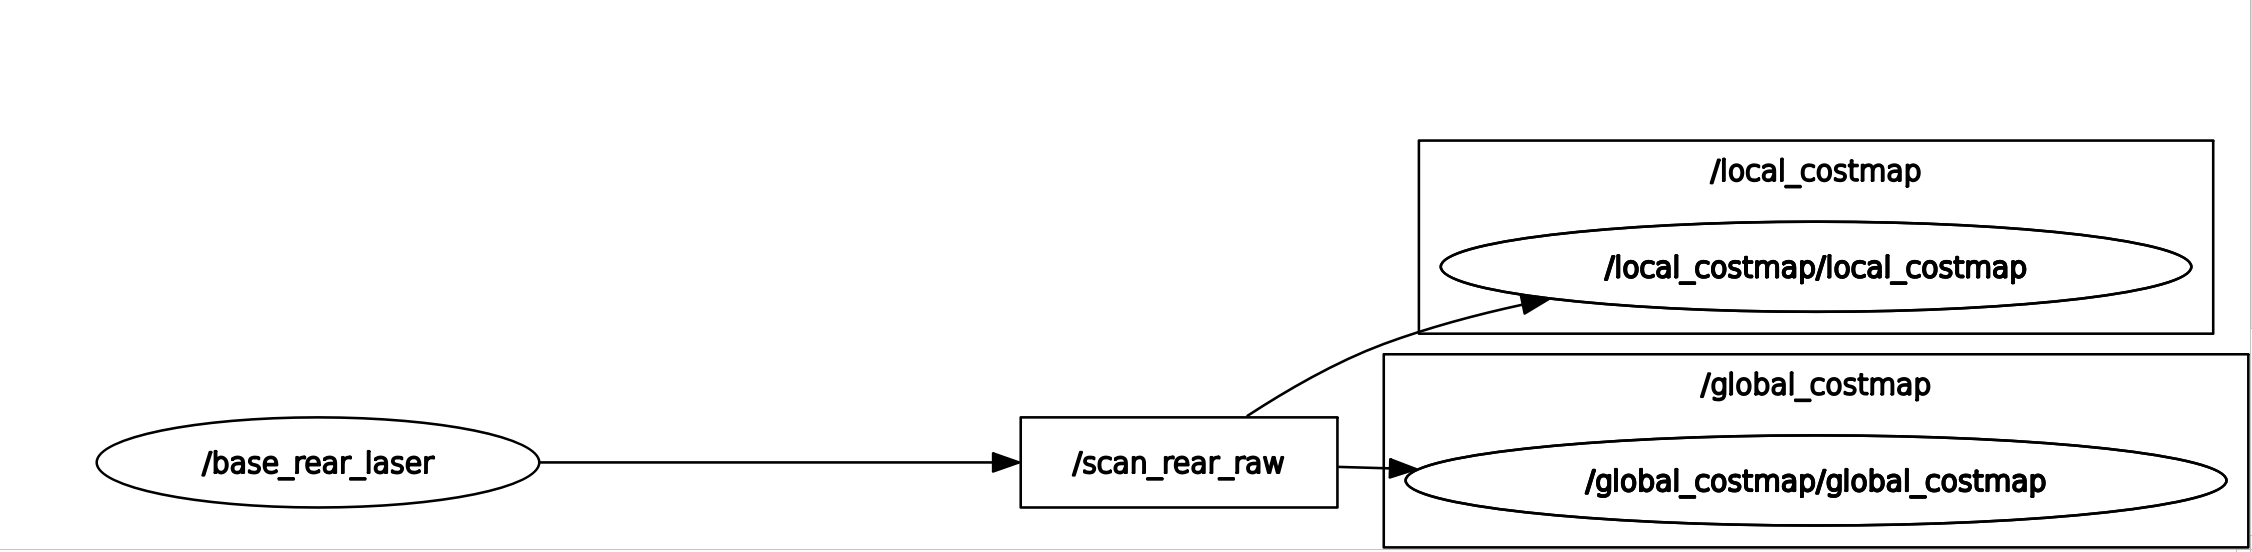
\includegraphics[width=1\textwidth]{images/Ch3/rosgraph_scan_rear.png}
    \caption{Data flow graphs of the OmniBase LiDAR sensors generated via \texttt{rqt\_graph}. Top: The front laser data is ingested by both the costmaps and the AMCL node. Bottom: The rear laser data is exclusively fused into the costmaps for 360-degree obstacle avoidance.}
    \label{fig:laser_graphs}
\end{figure}

Beyond obstacle avoidance, this sensory divergence heavily impacted the Adaptive Monte Carlo Localization (AMCL) system. By default, the PMB2 localization is governed by the \texttt{nav2\_amcl::DifferentialMotionModel}. To properly localize the holonomic base, the robot model type was explicitly switched to the \texttt{nav2\_amcl::OmniMotionModel}. 

This algorithmic switch requires a direct application of the probabilistic theories discussed in Section \ref{sec:probabilistic_motion_models}. In the differential model, the odometric noise is governed by four coefficients ($\alpha_1$ through $\alpha_4$), which model the variance of rotation and longitudinal translation. However, the Mecanum rollers of the OmniBase introduce continuous, controlled lateral slippage. To prevent the particle filter from diverging during lateral translations, the \texttt{alpha5} parameter was introduced into the AMCL configuration. As documented in the configuration files (provided in Appendix \ref{app:nav2_params}), \texttt{alpha5} was set to $0.2$, explicitly bounding the lateral variance ($\sigma^2_y$) and ensuring that the localization filter remained robust even during pure lateral strafing.

It is worth noting that the general holonomic odometry model derived in Section \ref{subsec:holonomic_uncertainty} employs nine coefficients ($\alpha_1$--$\alpha_9$) to describe the fully coupled error propagation across the $x$, $y$, and $\theta$ axes. The \texttt{nav2\_amcl::OmniMotionModel} implements a reduced, five-parameter form of this model ($\alpha_1$ -$\alpha_5$): the four differential coefficients $\alpha_1$--$\alpha_4$ are retained, and the additional $\alpha_5$ term accounts for the lateral (strafing) noise that the differential model omits. This reduced parameterisation is adequate in practice, since the dominant new contribution introduced by holonomic motion is precisely the lateral variance $\sigma_y^2$.

\subsection{Kinematic Constraints and Costmap Adaptation}
\label{subsec:costmap_tuning}

In the Nav2 architecture, the raw velocity commands generated by the local planner are not sent directly to the hardware base. Instead, they are routed through the \texttt{velocity\_smoother} node, which enforces strict kinematic limits, acceleration profiles, and deadbands. 

In the default PMB2 configuration, this smoother acts as a hard kinematic gatekeeper, strictly enforcing non-holonomic constraints. As documented in the configuration files (Appendix \ref{app:nav2_params}), the lateral component of the velocity limits for the differential base is explicitly clamped to zero (\texttt{max\_velocity: [1.0, 0.0, 1.0]} and \texttt{min\_velocity: [-1.0, 0.0, -1.0]}, the central entry being $v_y$). Consequently, even if a generic local planner attempted to output a lateral translation, the smoother would truncate the $v_y$ component, forcing the robot into a purely differential behavior. To physically unlock the kinematics for the OmniBase, these limits were symmetrically expanded (\texttt{max\_velocity: [1.0, 1.0, 1.0]} and \texttt{min\_velocity: [-1.0, -1.0, -1.0]}). Crucially, the minimum $X$ velocity was intentionally maintained at $-1.0$ across both platforms, rather than $0.0$, to ensure that the Nav2 \texttt{BackUp} recovery behavior could still operate effectively during collision avoidance.

Beyond velocity constraints, the geometric representation of the robot within the environment required a fundamental adaptation. The PMB2 operates with a perfectly circular static footprint, defined in both the \texttt{local\_costmap} and \texttt{global\_costmap} by a \texttt{robot\_radius} of $0.275$ meters. A circular footprint is computationally lightweight because its collision bounds are rotationally invariant. 

Conversely, the OmniBase necessitates a rectangular footprint (Figure~\ref{fig:footprints_rviz}) to accurately encapsulate its chassis and Mecanum wheels. The configuration was therefore modified from a scalar radius to a definitive polygon: \texttt{footprint: "[[0.35, 0.24], [-0.35, 0.24], [-0.35, -0.24], [0.35, -0.24]]"}. Introducing a rectangular footprint fundamentally alters the inflation layers and collision-checking heuristics of the costmaps. Because the corners of the rectangle extend further from the geometric center than the lateral sides, the local planner must strictly evaluate the robot's orientation relative to nearby obstacles, particularly during diagonal or pure lateral strafing maneuvers. To maintain adequate safety margins across both kinematics, the \texttt{inflation\_radius} in the local costmap was standardized to $0.55$ meters.

\begin{figure}[H]
    \centering
    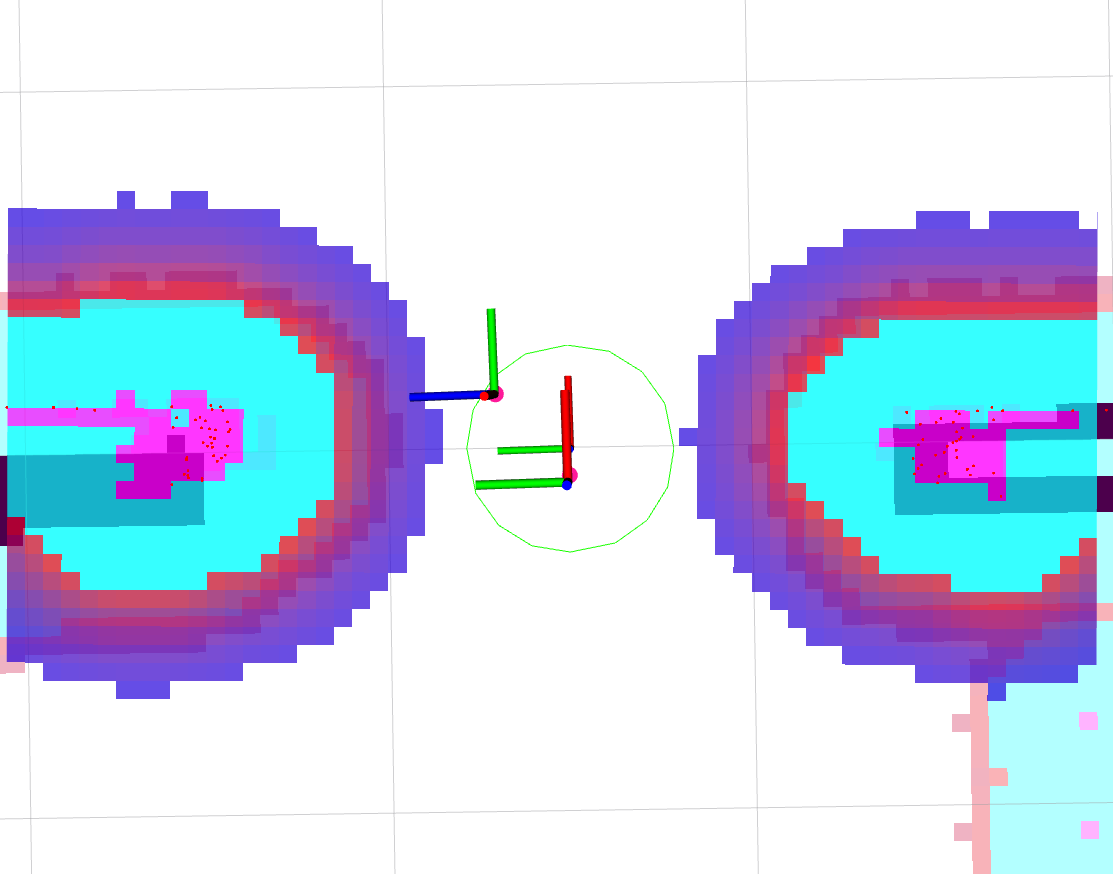
\includegraphics[width=0.48\textwidth]{images/Ch3/footprint_diff.png}
    \hfill
    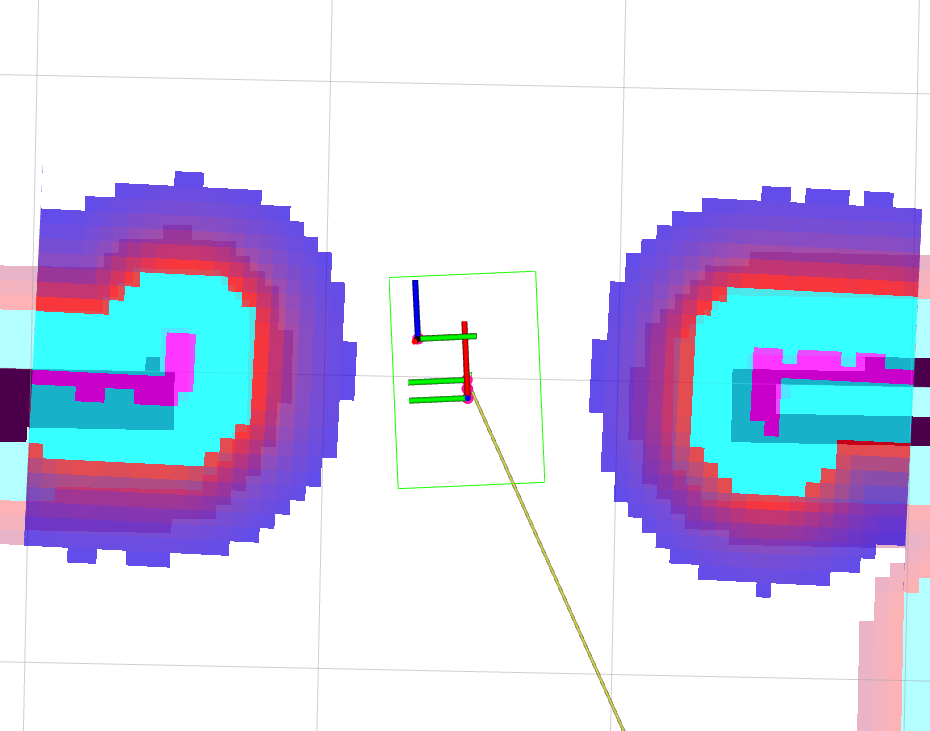
\includegraphics[width=0.48\textwidth]{images/Ch3/footprint_omni.png}
    \caption{Visualization of the local costmap and robot footprints in RViz located in a door. Left: The rotation-invariant circular footprint of the PMB2. Right: The rectangular footprint of the OmniBase.}
    \label{fig:footprints_rviz}
\end{figure}

\subsection{Overcoming the Differential Bias in the Local Planner}
\label{subsec:dwb_tuning}

The most significant architectural hurdle in deploying a holonomic robot within Nav2 lies in the interaction between the global and local planners. By default, the \texttt{NavfnPlanner} computes the optimal geometric path and automatically assigns an orientation to each intermediate pose that is strictly tangent to the trajectory. This inherently imposes a differential-drive advancement logic, dictating that the robot must continuously point its front face towards the direction of travel. 

The \texttt{DWBLocalPlanner} evaluates the feasibility of these trajectories using a set of cost functions known as \textit{Critics}. In the PMB2 baseline configuration, critics such as \texttt{PathAlign} and \texttt{GoalAlign} are heavily weighted (\texttt{scale: 32.0} and \texttt{24.0}, respectively). These critics heavily penalize any movement where the robot's heading does not match the trajectory tangent, effectively forcing the robot to rotate before translating. If applied to the OmniBase, this differential bias overrides its holonomic capabilities, resulting in sub-optimal, parabolic trajectories.

To unlock true omnidirectional movement—specifically, pure lateral translation or \textit{crab walking}—the critics evaluating the robot's heading were radically retuned. For the OmniBase, the weights of \texttt{PathAlign} and \texttt{GoalAlign} were strictly reduced to $0.0$ and $0.0$ (the complete configuration of the retuned Critics is detailed in Appendix \ref{app:dwb_tuning}). By suppressing the obligation to "look ahead", the planner is freed to command lateral velocities ($v_y \neq 0$) while maintaining the initial orientation. For these lateral commands to be resolved with sufficient granularity, the number of velocity samples along the $y$ axis was raised from the differential default (\texttt{vy\_samples: 5}) to \texttt{vy\_samples: 20}, matching the longitudinal resolution; otherwise the discretised velocity search would explore the lateral dimension too coarsely to yield smooth strafing. To ensure the robot did not drift from the optimal line, the \texttt{PathDist} scale was kept high ($64.0$), anchoring the chassis to the geometric path. 

Furthermore, a new critic, \texttt{Twirling} (\texttt{scale: 20.0}), was introduced to the holonomic configuration. Without orientation constraints, an unpenalized holonomic planner might generate arbitrary in-place rotations during lateral strafing. The \texttt{Twirling} critic actively penalizes unnecessary rotational velocities ($\omega$), forcing the robot to maintain a stable, fixed heading throughout the translation. Finally, matching the footprint adaptation discussed previously, the lightweight \texttt{BaseObstacle} critic used for the PMB2 was replaced with the computationally rigorous \texttt{ObstacleFootprint} critic, ensuring collision evaluations were strictly based on the actual rectangular polygon rather than an inscribed radius.

From an automation engineering perspective, forcing the OmniBase into a pure \textit{crab walk} provides two critical operational advantages:
\begin{enumerate}
    \item \textbf{Minimization of Swept Volume:} Pure translation maintains the robot's dynamic footprint strictly equal to its static footprint. By eliminating the need for parabolic turning and in-place rotations, the swept volume is drastically reduced, enabling safer and highly efficient navigation in cluttered or narrow environments.
    \item \textbf{Payload and Perception Stability:} By decoupling the chassis orientation from the velocity vector, the robot can maintain a continuous, fixed viewpoint on a target (e.g., keeping head-mounted optical sensors focused) or carry a manipulated payload steadily without requiring high-frequency compensatory movements from the upper-body joints.
\end{enumerate}

\subsection{Methodological Fairness and Configuration Summary}
\label{subsec:fairness_summary}

A critical methodological declaration must be made regarding the comparative validity of this experimental setup. In robotic benchmarking, applying an identical configuration file to fundamentally distinct hardware platforms does not guarantee an objective comparison; rather, it forces one platform to operate under the physical paradigms of the other. 

To ensure true methodological fairness, each base was explicitly tuned to exploit its own specific kinematics. As summarized in Table \ref{tab:nav2_params}, parameters directly related to the controllable degrees of freedom (such as lateral velocity limits) and heuristic orientation critics (\texttt{PathAlign}, \texttt{GoalAlign}, and \texttt{Twirling}) deliberately differ between the configurations. These kinematic-specific divergences were implemented by design to eliminate the differential bias and unlock the OmniBase's capabilities. 

Conversely, to prevent incidental misalignments from skewing the results, all hardware-agnostic parameters—including maximum linear and angular velocities, acceleration profiles, inflation radii, and path-tracking weights (\texttt{PathDist})—were strictly standardized across both bases. By isolating the parameters in this manner, it is guaranteed that the performance differences observed in the subsequent experimental campaigns derive exclusively from the underlying kinematic properties and the resulting navigation strategies, rather than from arbitrary configuration noise.

\begin{table}[htbp]
    \centering
    \renewcommand{\arraystretch}{1.3}
    \caption{Summary of critical Nav2 parameters highlighting the intentional divergences and standardized similarities between the PMB2 and OmniBase configurations.}
    \vspace{0.2cm}
    \label{tab:nav2_params}
    \begin{tabularx}{\textwidth}{@{} l l l >{\raggedright\arraybackslash}X @{}}
        \toprule
        \textbf{Parameter Name} & \textbf{PMB2 (Diff)} & \textbf{OmniBase (Omni)} & \textbf{Rationale} \\
        \midrule
        \multicolumn{4}{c}{\textbf{Kinematic-Specific Parameters (Tuned by Design)}} \\
        \midrule
        Lateral Vel ($v_y$) & \texttt{[0.0, 0.0]} & \texttt{[-1.0, 1.0]} & Unlocks lateral strafing ($Y$-axis). \\
        Velocity Samples ($v_y$) & \texttt{5} & \texttt{20} & Finer lateral sampling for smooth strafing. \\
        Footprint Geometry & \texttt{radius: 0.275} & \texttt{polygon: [...]} & Matches physical chassis geometry. \\
        \texttt{PathAlign} Critic & \texttt{scale: 32.0} & \texttt{scale: 0.0} & Suppresses forward-heading bias. \\
        \texttt{GoalAlign} Critic & \texttt{scale: 24.0} & \texttt{scale: 0.0} & Decouples orientation from motion. \\
        \texttt{Twirling} Critic & Not utilized & \texttt{scale: 20.0} & Penalizes arbitrary spin during strafe. \\
        AMCL Motion Model & \texttt{Differential} & \texttt{OmniMotion} & Matches probabilistic mechanics. \\
        AMCL \texttt{alpha5} Noise & Not evaluated & \texttt{0.2} & Bounds lateral slippage variance. \\
        \midrule
        \multicolumn{4}{c}{\textbf{Identical Parameters (Standardized Baseline)}} \\
        \midrule
        Max Vel ($v_x$, $\omega$) & \texttt{1.0, 1.0} & \texttt{1.0, 1.0} & Standardized absolute speed limits. \\
        Max Accel ($a_x$, $a_\omega$) & \texttt{2.5, 3.2} & \texttt{2.5, 3.2} & Standardized dynamic constraints. \\
        \texttt{PathDist} Critic & \texttt{scale: 64.0} & \texttt{scale: 64.0} & Equal adherence to global trajectory. \\
        \texttt{GoalDist} Critic & \texttt{scale: 24.0} & \texttt{scale: 24.0} & Equal attraction to the final goal. \\
        \texttt{inflation\_radius} & \texttt{0.55} & \texttt{0.55} & Consistent obstacle safety margin. \\
        AMCL $\alpha_1 - \alpha_4$ & \texttt{0.2} & \texttt{0.2} & Consistent base odometric noise. \\
        \bottomrule
    \end{tabularx}
\end{table}